% Created 2021-10-08 Fri 08:57
% Intended LaTeX compiler: pdflatex
\documentclass[presentation,aspectratio=169, usenames, dvipsnames]{beamer}
\usepackage[utf8]{inputenc}
\usepackage[T1]{fontenc}
\usepackage{graphicx}
\usepackage{grffile}
\usepackage{longtable}
\usepackage{wrapfig}
\usepackage{rotating}
\usepackage[normalem]{ulem}
\usepackage{amsmath}
\usepackage{textcomp}
\usepackage{amssymb}
\usepackage{capt-of}
\usepackage{hyperref}
\usepackage{khpreamble}
\usepackage{amssymb}
\usepgfplotslibrary{groupplots}
\newcommand*{\shift}{\operatorname{q}}
\definecolor{ppc}{rgb}{0.1,0.1,0.6}
\definecolor{iic}{rgb}{0.6,0.1,0.1}
\definecolor{ddc}{rgb}{0.1,0.6,0.1}
\def\ucolor{blue!80!black}
\def\ycolor{green!60!black}
\newcommand*{\incolor}[1]{\textcolor{\ucolor}{#1}}
\newcommand*{\outcolor}[1]{\textcolor{\ycolor}{#1}}
\usetheme{default}
\author{Kjartan Halvorsen}
\date{\today}
\title{PID for industrial control}
\hypersetup{
 pdfauthor={Kjartan Halvorsen},
 pdftitle={PID for industrial control},
 pdfkeywords={},
 pdfsubject={},
 pdfcreator={Emacs 26.3 (Org mode 9.4.6)}, 
 pdflang={English}}
\begin{document}

\maketitle

\section{PID tuning - (Smith and Corripio) Ziegler Nichols}
\label{sec:org7d5d788}
\begin{frame}[label={sec:orgb4c1428}]{The PID - practical form}
\definecolor{ppc}{rgb}{0.1,0.1,0.6}
\definecolor{iic}{rgb}{0.6,0.1,0.1}
\definecolor{ddc}{rgb}{0.1,0.5,0.1}

\begin{center}
  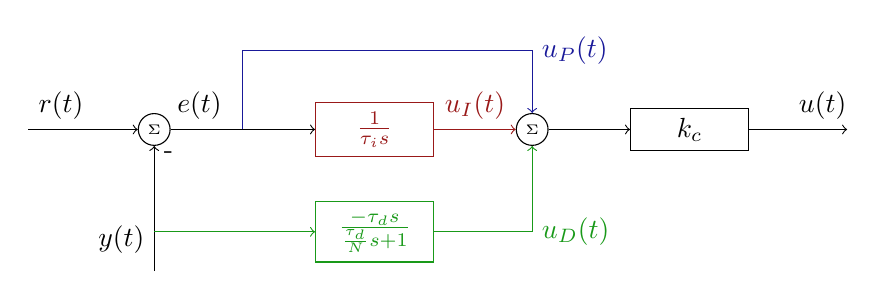
\begin{tikzpicture}[node distance=22mm, block/.style={rectangle, draw, minimum width=15mm}, sumnode/.style={circle, draw, inner sep=2pt}]

    \node[coordinate] (input) {};
    \node[sumnode, right of=input, node distance=16mm] (sum) {\tiny $\Sigma$};
    \node[color=iic,block, right of=sum, node distance=28mm] (ii)  {$\frac{1}{\tau_is}$};
    \node[color=ppc, coordinate, above of=ii, node distance=10mm] (pp)  {};
    \node[color=ddc,block, below of=ii, node distance=13mm] (dd)  {$\frac{-\tau_ds}{\frac{\tau_d}{N}s + 1}$};
    \node[sumnode, right of=ii, node distance=20mm] (sum2) {\tiny $\Sigma$};
    \node[block, right of=sum2, node distance=20mm] (gain)  {$k_c$};
    \node[coordinate, below of=sum, node distance=18mm] (feedback) {};
    \node[coordinate, right of=gain, node distance=20mm] (output) {};

    \draw[->] (input) -- node[above, pos=0.3] {$r(t)$} (sum);
    \draw[->] (sum) -- node[above, pos=0.2] {$e(t)$} node[coordinate] (mm) {}  (ii);
    \draw[->] (gain) -- node[above, near end] {$u(t)$} (output);
    \draw[->] (feedback) -- node[left, near start] {$y(t)$} node[right, pos=0.95] {-} (sum);
    \draw[->, color=ppc] (mm) |- (pp) -| node[right,] {$u_P(t)$} (sum2);
    \draw[->, color=ddc] (feedback |- dd) -- node[above, pos=0.95] {} (dd);
    \draw[->, color=ddc] (dd) -| node[right,] {$u_D(t)$} (sum2)  ;
    \draw[->, color=iic] (ii)  -- node[above,] {$u_I(t)$} (sum2);
    \draw[->] (sum2) -- node[above, near end] {} (gain);

  \end{tikzpicture}
\end{center}

\alert{Activity} What are the modifications and why are they introduced, comparing to the controller \(F(s) = k_c\left(1 + \frac{1}{\tau_i s} + \tau_d s\right)\)?
\end{frame}

\begin{frame}[label={sec:org168e46f}]{PID tuning}
\end{frame}
\begin{frame}[label={sec:org974319e}]{Method by Smith \& Corripio using table by Ziegler-Nichols}
\small

Given process model (fitted to response of the system) \[ G(s) = K \frac{\mathrm{e}^{-s\theta}}{\tau s + 1} \] and PID controller
   \[ F(s) = k_c\left( 1 + \frac{1}{\tau_i s} + \tau_d s\right) \]
   Choose the PID parameters according to the following table (Ziegler-Nichols, 1943)
   \begin{center}
   \setlength{\tabcolsep}{20pt}
   \renewcommand{\arraystretch}{1.5}
   \begin{tabular}{llll}
   Controller & \(k_c\) & \(\tau_i\) & \(\tau_d\)\\
  \hline\hline
  P & \(\frac{\tau}{\theta K}\) &  & \\
  PI & \(\frac{0.9\tau}{\theta K}\) & \(\frac{\theta}{0.3}\) & \\
  PID & \(\frac{1.2\tau}{\theta K}\) & \(2\theta\) & \(\frac{\theta}{2}\)\\
  \hline
\end{tabular}
\end{center}

Gives good control for \[0.1 < \frac{\theta}{\tau} < 0.6.\]
\end{frame}


\section{The delay transfer function}
\label{sec:org13c8ece}

\begin{frame}[label={sec:org4fe7098}]{The delay}
\begin{center}
  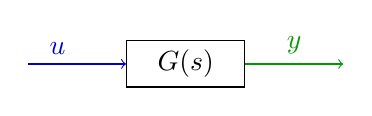
\begin{tikzpicture}[scale = 0.8, node distance=20mm, block/.style={rectangle, draw, minimum width=15mm}, sumnode/.style={circle, draw, inner sep=2pt}]

  \node[coordinate] (refinput) {};
  \node[block, right of=refinput] (motor) {$G(s)$};
  \node[coordinate, right of=motor, node distance=20mm] (output) {};

  \draw[\ucolor, ->] (refinput) -- node[above, pos=0.3] (voltsignal) {$u$} (motor);
  \draw[\ycolor, ->] (motor) -- node[above, pos=0.5] (velsignal) {$y$} (output);
  \end{tikzpicture}
\end{center}

Let \(\incolor{u(t) = \sin\omega_1 t}\). Then, after transients have died out,
\[ \outcolor{y(t)}= \outcolor{|G(\omega_1)| \sin \big( \omega_1 t + \arg G(i\omega_1)\big)}. \]

\pause
\alert{If ouput is simply a delayed input} \(\outcolor{y(t)}= \outcolor{ \sin \big( \omega_1 (t - \theta) \big)}\)

\pause
\alert{Activity} 
Identify \(|G(i\omega)|\) and \(\arg G(i\omega)\) for the pure delay.
\end{frame}

\begin{frame}[label={sec:org3ad6758}]{The Bode-plot of the delay}
\begin{columns}
\begin{column}{0.7\columnwidth}
\begin{center}
  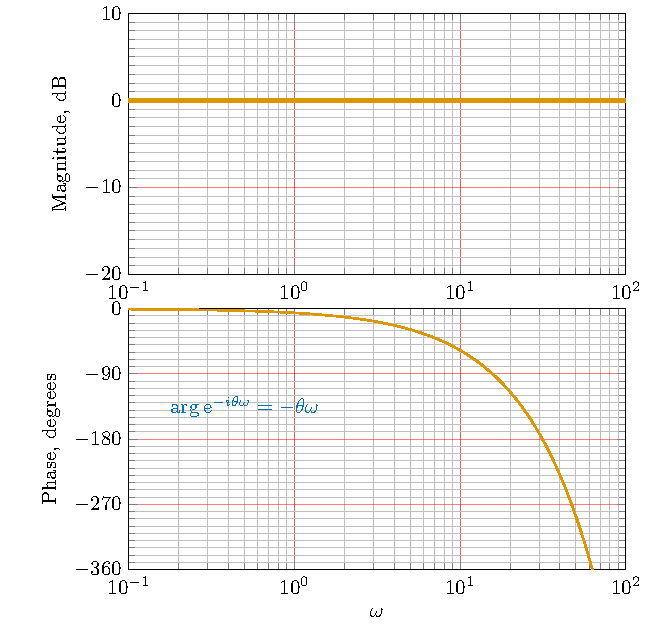
\includegraphics[width=.8\linewidth]{../../figures/bode-delay}
\end{center}
\end{column}

\begin{column}{0.6\columnwidth}
\pause

\alert{Review of Excercises for Session 3}

What is the time-delay \(\theta\)?
\end{column}
\end{columns}
\end{frame}

\section{Analytical PID design}
\label{sec:org90ed2bc}

\begin{frame}[label={sec:org5b54ab8}]{Analytical PID design}
\end{frame}
\begin{frame}[label={sec:org3701623}]{Analytical PID design}
   \begin{center}
   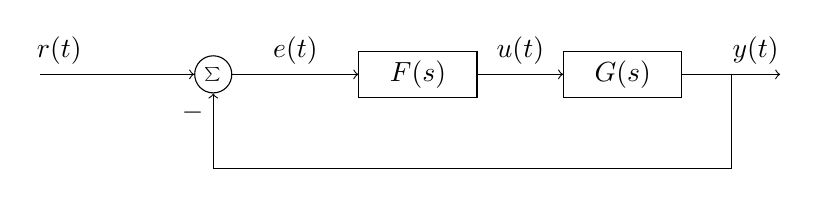
\begin{tikzpicture}[node distance=22mm, block/.style={rectangle, draw, minimum width=15mm}, sumnode/.style={circle, draw, inner sep=2pt}]
  { 
  \node[coordinate] (input) {};
  \node[sumnode, right of=input] (sum) {\tiny $\sum$};
  \node[block, right of=sum, node distance=2.6cm] (reg) {$F(s)$};
  \node[block, right of=reg, node distance=2.6cm] (plant) {$G(s)$};
  \node[coordinate, right of=plant, node distance=2cm] (output) {};
  \node[coordinate, below of=plant, node distance=12mm] (feedback) {};
 
  \draw[->] (plant) -- node[coordinate, inner sep=0pt] (meas) {} node[near end, above] {$y(t)$} (output);
  \draw[->] (meas) |- (feedback) -| node[very near end, left] {$-$} (sum);
  \draw[->] (input) -- node[very near start, above] {$r(t)$} (sum);
  \draw[->] (sum) -- node[above] {$e(t)$} (reg);
  \draw[->] (reg) -- node[above] {$u(t)$}(plant);
}
\end{tikzpicture}
\end{center}

\alert{Activity}  Solve for \(F(s)\) in the closed-loop transfer function \[G_c(s) = \frac{G(s)F(s)}{1 + G(s)F(s)}\] 
\end{frame}

\begin{frame}[label={sec:orga5c28fe}]{Analytical PID design - Solution}
\end{frame}
\begin{frame}[label={sec:org99ec3bb}]{Analytical PID design - Solution}
Solving for \(F(s)\) in the closed-loop transfer function \(G_c(s) = \frac{G(s)F(s)}{1 + G(s)F(s)}\) 

\[ \big(1 + G(s)F(s)\big) G_c(s) = G(s)F(s)\]
\[ G_c(s) = \big( 1 - G_c(s)\big) G(s)F(s)\]
\[F(s) = \frac{\frac{G_c(s)}{G(s)}}{1 - G_c(s)}\]
\end{frame}

\begin{frame}[label={sec:orgb8e67b6}]{Analytic PID tuning - first-order with delay}
   \begin{center}
   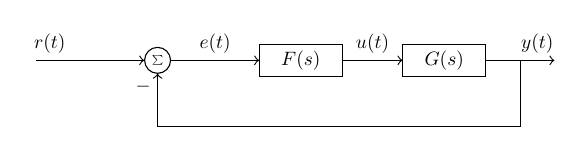
\begin{tikzpicture}[scale=0.7, transform shape, node distance=22mm, block/.style={rectangle, draw, minimum width=15mm}, sumnode/.style={circle, draw, inner sep=2pt}]
  { 
  \node[coordinate] (input) {};
  \node[sumnode, right of=input] (sum) {\tiny $\sum$};
  \node[block, right of=sum, node distance=2.6cm] (reg) {$F(s)$};
  \node[block, right of=reg, node distance=2.6cm] (plant) {$G(s)$};
  \node[coordinate, right of=plant, node distance=2cm] (output) {};
  \node[coordinate, below of=plant, node distance=12mm] (feedback) {};
 
  \draw[->] (plant) -- node[coordinate, inner sep=0pt] (meas) {} node[near end, above] {$y(t)$} (output);
  \draw[->] (meas) |- (feedback) -| node[very near end, left] {$-$} (sum);
  \draw[->] (input) -- node[very near start, above] {$r(t)$} (sum);
  \draw[->] (sum) -- node[above] {$e(t)$} (reg);
  \draw[->] (reg) -- node[above] {$u(t)$}(plant);
}
\end{tikzpicture}
\end{center}

Given model \(G(s) = K \frac{\mathrm{e}^{-s\theta}}{\tau s + 1}\) of the process and desired closed-loop transfer function \(G_c(s) = \frac{\mathrm{e}^{-s\theta}}{\tau_c s + 1}\)

\begin{align*}
F(s) &=  \frac{ \frac{G_c(s)}{G(s)}}{1 - G_c(s)} = \frac{ \frac{\mathrm{e}^{-s\theta}}{\tau_cs + 1} \frac{\tau s + 1}{K \mathrm{e}^{-s\theta}} }{1 - \frac{\mathrm{e}^{-s\theta}}{\tau_cs + 1}} = \frac{1}{K} \left( \frac{\tau s + 1}{\tau_c s + 1 - \mathrm{e}^{-s\theta}} \right) \\
&\approx \frac{1}{K} \left( \frac{\tau s + 1}{(\tau_c+\theta) s}\right)
%  = \underbrace{\frac{\tau}{K(\tau_c+\theta)}}_{k_c} \left( 1 + \frac{1}{\underbrace{\tau}_{\tau_i} s} \right).
\end{align*}

\pause
\alert{Activity}  A PI-controller can be written \(F(s) = k_c\frac{\tau_is + 1}{\tau_i s}\). Determine \(k_c\) and \(\tau_i\) in terms of the parameters \(K\), \(\theta\), \(\tau\) and \(\tau_c\). 
\end{frame}

\begin{frame}[label={sec:org9f32e07}]{Example}
   \begin{center}
   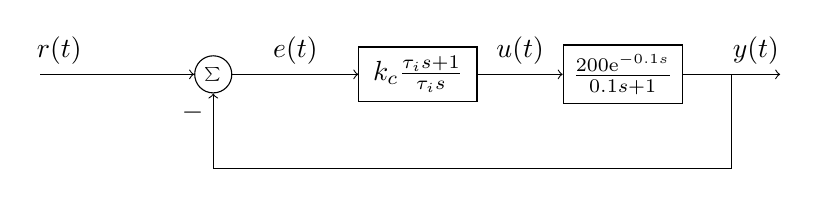
\begin{tikzpicture}[node distance=22mm, block/.style={rectangle, draw, minimum width=15mm}, sumnode/.style={circle, draw, inner sep=2pt}]
  { 
  \node[coordinate] (input) {};
  \node[sumnode, right of=input] (sum) {\tiny $\sum$};
  \node[block, right of=sum, node distance=2.6cm] (reg) {$k_c\frac{\tau_i s + 1}{\tau_i s}$};
  \node[block, right of=reg, node distance=2.6cm] (plant) {$\frac{200 \mathrm{e}^{-0.1s}}{0.1s + 1}$};
  \node[coordinate, right of=plant, node distance=2cm] (output) {};
  \node[coordinate, below of=plant, node distance=12mm] (feedback) {};
 
  \draw[->] (plant) -- node[coordinate, inner sep=0pt] (meas) {} node[near end, above] {$y(t)$} (output);
  \draw[->] (meas) |- (feedback) -| node[very near end, left] {$-$} (sum);
  \draw[->] (input) -- node[very near start, above] {$r(t)$} (sum);
  \draw[->] (sum) -- node[above] {$e(t)$} (reg);
  \draw[->] (reg) -- node[above] {$u(t)$}(plant);
}
\end{tikzpicture}
\end{center}

\(k_c = \frac{\tau}{K(\tau_c+\theta)}\) and \(\tau_i = \tau\).

\alert{Activity} Determine the controller for the choice \(\tau_c = \tau\)
\end{frame}



\begin{frame}[label={sec:org7cb52e1}]{The PID - practical aspects}
{\footnotesize Åström \& Hägglund (1988) \emph{PID controllers: Theory, design and tuning, 2nd ed} Instrument Society of America.}

\begin{block}{Approximating nonlinear systems with linear models}
\begin{itemize}
\item Model is accurate only in neighborhood of operating point for which the system is approximated.
\item Solution: Divide operating range into many regions, with separate PID parameters for each region
\end{itemize}
\end{block}

\begin{block}{Approximating high-order systems with low-order models}
\begin{itemize}
\item Only accurate for low frequencies
\item Beware of behavior for high-frequency input to the closed-loop system
\end{itemize}
\end{block}
\end{frame}

\begin{frame}[label={sec:org348d7d8}]{The PID - practical aspects, contd}
\begin{block}{When do PID controllers work well?}
\begin{itemize}
\item The plant dynamics can be well approximated with low-order model
\item Demands on performance not too high
\end{itemize}
\end{block}
\begin{block}{More sophisticated control needed when}
\begin{itemize}
\item Higher order dynamics
\item Oscillatory modes
\item Long deadtime
\end{itemize}
\end{block}
\end{frame}

\begin{frame}[label={sec:org8734794}]{The PID - practical aspects, contd}
\begin{block}{Choice of controller}
\begin{enumerate}
\item P-controller if damping and steady-state error satisfied
\item PI-controller if steady-state error must be zero (often 1st order dynamics)
\item PID-controller if PI does not give sufficient damping (often 2nd order dynamics)
\item Tuning parameter \(\tau_c\) for SIMC tuning method: 
\begin{itemize}
\item Smaller (=faster) than \(\tau\) if sufficiently damped and limitations on input signal not violated.
\item larger (=slower) than \(\tau\) if more damping required or smaller input signal required.
\end{itemize}
\end{enumerate}
\end{block}
\end{frame}



\section{Windup}
\label{sec:orgcbf51b3}

\begin{frame}[label={sec:org74f2e63}]{Integral windup}
\end{frame}

\section{Anti-windup}
\label{sec:orgc2e60f9}

\begin{frame}[label={sec:org9814f48}]{Anti-windup using back-calculation}
\begin{center}
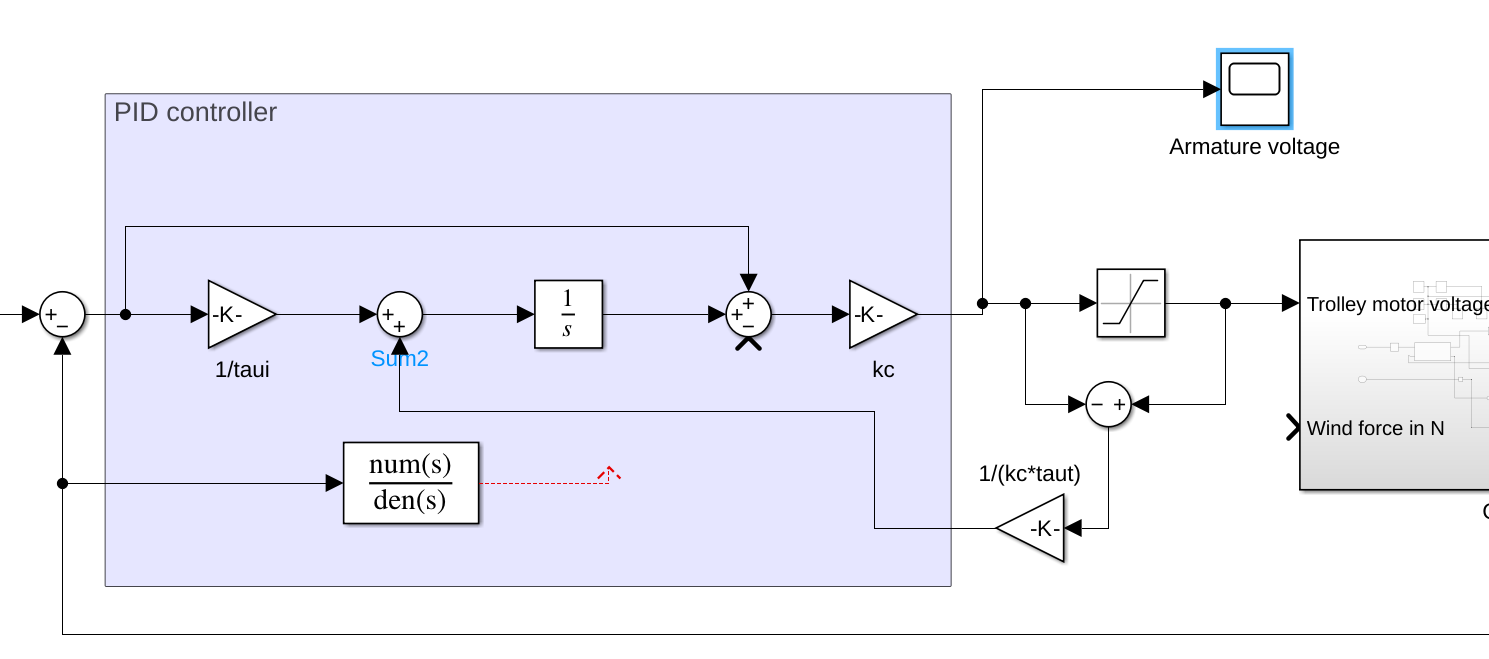
\includegraphics[width=.7\linewidth]{/home/kjartan/tec/mr2025/figures/Simulink-backtracking.png}
\end{center}
\end{frame}

\begin{frame}[label={sec:org251c356}]{Anti-windup using back-calculation}
   \begin{center}
 	  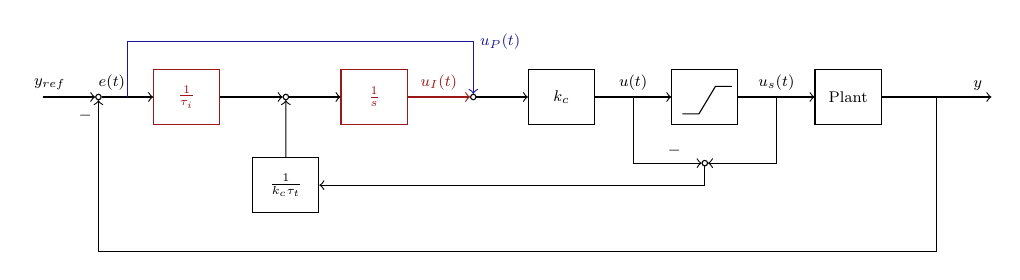
\begin{tikzpicture}[every node/.append style={transform shape}, scale = 0.7, font=\footnotesize,
	block/.style={rectangle, draw, minimum width=12mm, minimum height=10mm, inner sep=4pt},
	amp/.style = {regular polygon, regular polygon sides=3,
              draw, fill=white, text width=1em,
              inner sep=1pt, outer sep=0mm,
              shape border rotate=-90},
	      summ/.style = {circle, draw, inner sep = 1pt},]
	 \node[block, align=center] (motor) at (0,0) {Plant};
	 \node[coordinate, right of=motor, node distance = 26mm,] (output) {};
	 \node[block, left of=motor, node distance=26mm] (saturation) {};

	 \node[block, left of=saturation, node distance=26mm] (gain)  {$k_{c}$};
	 
	 \node[summ, left of=gain, node distance=16mm] (sum2) {};
	 \node[color=iic,block, left of=sum2, node distance=18mm] (int)  {$\frac{1}{s}$};
	 \node[summ, left of=int, node distance=16mm] (sumint) {};
	 \node[color=iic,block, left of=sumint, node distance=18mm] (ii)  {$\frac{1}{\tau_{i}}$};
	 \node[color=ppc, coordinate, above of=ii, node distance=10mm] (pp)  {};
	 \node[summ, left of=ii, node distance=16mm] (sumsp) {};
	 \node[coordinate, left of=sumsp, node distance = 10mm,] (setpoint) {};

       \draw[->] (sumsp) -- node[above, pos=0.2] {$e(t)$} node[coordinate] (mm) {}  (ii);
       \draw[->] (gain) -- node[coordinate] (idmeas) {} node[above, ] {$u(t)$} (saturation);
       \draw[->, color=ppc] (mm) |- (pp) -| node[right,] {$u_P(t)$} (sum2);
       \draw[->, color=iic] (int)  -- node[above,] {$u_I(t)$} (sum2);
       \draw[->] (sum2) -- node[above, near end] {} (gain);



	 \draw[->] (setpoint) -- node[above, very near start ] {$y_{ref}$} (sumsp);
	 \draw[->] (saturation) -- node[coordinate, ] (satmeas) {} node[above,] {$u_s(t)$} (motor);
	 \draw[->] (motor) -- node[coordinate] (meas) {} node[above, very near end] {$y$} (output);
	 \draw[->] (meas) -- node[right] {} ++(0,-28mm) -| node[pos=0.95, left] {$-$} (sumsp);

	 % Anti-windup
	 \draw ($ (saturation.south west) + (2mm, 2mm) $) -- ++(3mm, 0) -- ++(3mm, 5mm) -- ++(3mm, 0);
	 \node[block, below of=sumint, node distance=16mm] (back) {$\frac{1}{k_{c}\tau_t}$};
	 \node[summ, below of=saturation, node distance=12mm] (sumsat) {};
	 \draw[->] (satmeas) |- node[above, pos=0.8] {} (sumsat);
	 \draw[->] (idmeas) |- node[above, pos=0.8] {$-$} (sumsat);
	 \draw[->] (sumsat) |- (back);
	 \draw[->] (back) -- (sumint);
	 \draw[->] (ii) -- (sumint);
	 \draw[->] (sumint) -- (int);
	 

	 \node[coordinate, right of=back, node distance=2cm] (sat) {};
  
\end{tikzpicture}
\end{center}

\alert{Activity} Assume that the actuator is saturated. determine the transfer function from \(u_s(t)\) to \(u(t)\).
\end{frame}
\end{document}